\documentclass[10pt,a4paper]{article}
\usepackage[utf8]{inputenc}
\usepackage[italian]{babel}
\usepackage{amsmath}
\usepackage{amsfonts}
\usepackage{amssymb}
\usepackage{graphicx}
\usepackage{gensymb}
\usepackage[left=2cm,right=2cm,top=2cm,bottom=2cm]{geometry}
\newcommand{\rem}[1]{[\emph{#1}]}

\author{Gruppo BN \\Lisa Bedini,  Federico Belliardo, Marco Costa}
\title{Esperienza 15: Misura della costante di Boltzmann}

\begin{document}
\maketitle
\section{Scopo dell'esperienza}
Misurare la costante di Bolzmann dal rumore termico (Johnson-Nyquist) di una resistenza a temperatura nota, grazie ad un amplificator, un filtro passa-banda e un convertitore RMS.

\section{Materiale a disposizione}
\begin{itemize}
\item INA114 Amplificatore
\item AD708: OpAmp integrati
\item AD736: RMS converter
\end{itemize}

\section{Montaggio del circuito}
\subsection{Power filter}
La tensione di alimentazione (positive e negative) sono state filtrate mediante circuiti passa-basso prima di fornirle agli integrati in modo da ridurne le fluttuazioni:\\

\begin{figure}[!htb]
\centering
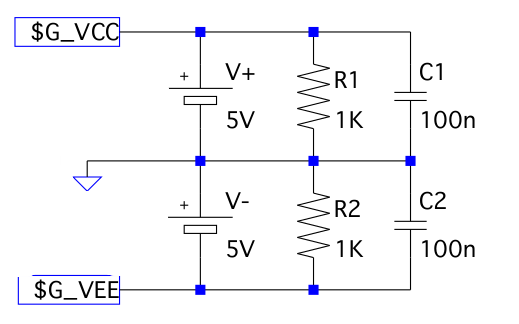
\includegraphics[scale=0.5]{powerfilter.png}
\caption{Filtri passa basso per le alimentazioni.\label{power}}
\end{figure}


\subsection{Preamplificatore}
Il primo stadio di amplificazione è stato realizzato con un \emph{Precision instrumentation amplifier} avente un guadagno atteso: $G_1 = 1+\frac{50 k\Omega}{1 k\Omega} = 51$. Il secondo stadio è un semplice amplificatore invertente con guadagno teorico $G_2 = \frac{68 k\Omega}{4.7 k\Omega} = 14.5$. Il valore ateso dell'amplificazione complessiva è: $A_1 = 740$.
%TODO 
Non sono stati propagati gli errori sulle resistenze per stimare l'incertezza sul guadagno teorico. Si nota che anche volendo farlo non conosciamo la precisione sulla calibrazione della resistenza interna dall'INA114.\\

\begin{figure}[!htb]
\centering
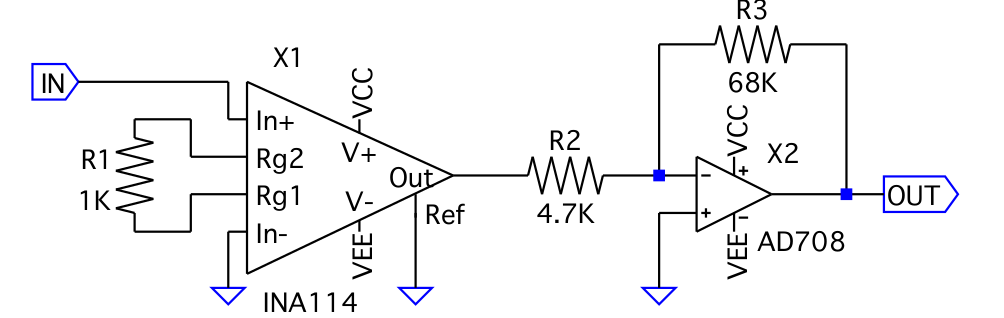
\includegraphics[scale=0.5]{preamp.png}
\caption{Preamplificatore realizzato con opAmp e INA114.\label{preamp}}
\end{figure}

Il circuito è stato analizzato fornendo in ingresso con il generatore di funzioni un onda sinusoidale di piccola ampiezza ($V_0 = $) e se ne è costruito il diagramma di Bode, come visualizzato in figura \fig{bode}. Esso si comporta come un filtro passa basso con una frequenza di taglio $f_t = $. Il segnale in uscita appare molto rumoroso.\\


\subsection{Filtro passa-banda e post amplificatore}
Si sono realizzati il filtro passa-banda e il post amplificatore come mostrato nelle figure.

\begin{figure}[!htb]
\centering
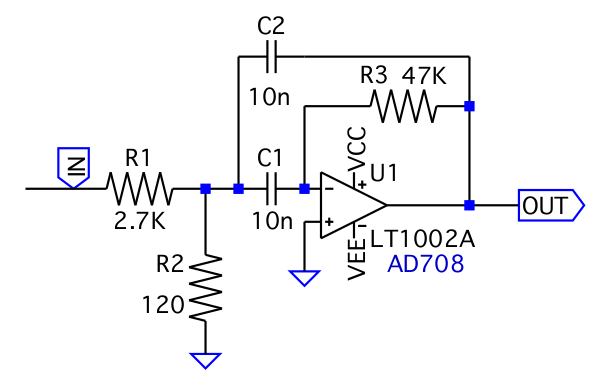
\includegraphics[scale=0.5]{banda.png}
\caption{Filtro passa-banda realizzato con opAmp.\label{banda}}
\end{figure}


\begin{figure}[!htb]
\centering
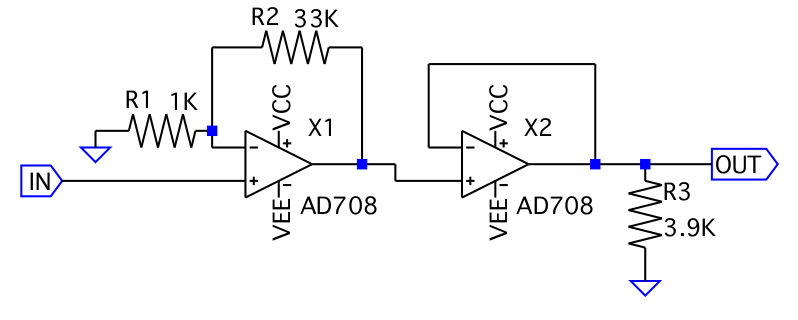
\includegraphics[scale=0.5]{postamp.png}
\caption{Post amplificatore realizzato con opAmp.\label{postamp}}
\end{figure}

L'analisi teorica del circuito passa-banda indica che questo ha una amplificazione massima $A_{banda} = \frac{R_3}{2 R_1} = 8.7$ in corrispondenza della frequenza $f_t = \frac{1}{2 \pi C} \sqrt{\frac{\frac{1}{R_1} + \frac{1}{R_2}}{R_3}} = 6.4 kHz$. La larghezza i banda prevista è: $\Delta f = \frac{1}{\pi R_3 C}$, agli estremi della quale l'amplificazione è di $3 dB$ inferiore a quella di picco. Il post amplificatore ha invece un guadagno $A_{post} = 1 + \frac{R_2}{R_1} = 34$, come è ben noto.l'amplificazione a centro banda attesa sarebbe dunque $A_{2} = A_{banda} A_{post} = 269$.\\

%TODO --> Finire....
E' stato realizzato un plot di Bode per questa parte di circuito e si sono confrontate le previsioni teoriche con le misure. Né l'amplificazione massima né la larghezza di banda misurate sono compatibili con quanto atteso. Questo è probabilmente dovuto a poli dell'opAmp (non idealità) che non sono ovviamente stati considerati.\\

Non è stato eseguito il fit di questo Bode.\\

In conclusione l'amplificazione totale del circuito, ottenuta moltiplicando i guadagni di tutti gli amplificatori misurati è: $A_0 = A_1 A_2 = $, qui riportata perché usata nei calcoli seguenti.\\

\subsection{Convertitore RMS}
L'ultima parte del circuito ha lo scopo di trasformare un segnale alternato in un segnale continuo restituendone il valore quadratico medio ed è stato realizzato con l'apposito integrato nel circuito riportato in figura:

\begin{figure}[!htb]
\centering
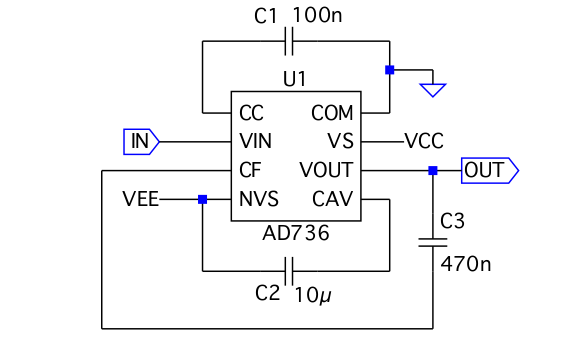
\includegraphics[scale=0.5]{rms.png}
\caption{Circuito RMS realizzato con appostito integrato.\label{rms}}
\end{figure}

\section{Misura della costante di Boltzmann}
%TODO ---> FINIRE
Il rumore ($V_{rms})$ totale è determinato dalla somma in quadratura dei rumori associati alla resistenza e quelli dovuti all'amplificatore, parametrizzati come rumori in serie e in parallelo all'amplificatore. Dalla teoria ci aspettiamo dunque: $V_{rms} = V_0 \sqrt{1+\frac{R}{R_t}+(\frac{R}{R_n})^2}$ dove:
\begin{itemize}
\item $V_0$ è il rumore in uscita a resistenza nulla (dato solo dal rumore in serie all'amplificatore)
\item $R_t = \frac{V_0^2}{4 k_b T A_0^2 \Delta f}$ è la resistenza equivalente del rumore in serie sull'ingresso dell'amplificatore (resistenza che genererebbe un rumore termico equivalente). Il parametro $A_0$ è l'amplificazione totale del circuito utilizzato (misurata), $\Delta f$ è la larghezza di banda del circuito (a cui si suppone contribuisca solo il passabanda), $T$ è ovviamente la temperatura ambiente.\\
\item $R_n$ è il rapporto tra il rumore in parallelo e il rumore in serie dell'amplificatore. E' chiaro che il rumore in parallelo (a differenza del rumore in serie) è presente solamente se vi è una resistenza ai capi dell'ingresso dell'amplificatore.\\ %Casi resitenza infinta e nulla non tonao proprio ma non scrivere
\end{itemize}

%Inserire parte relativa al fit...

Invertendo la formula per $R_t$ otteniamo: $k_B = \frac{V_0^2}{4 R_t T A_0^2 \Delta f} = $.

L'ordine di grandezza ottenuto per la costante di Boltzmann è corretto.\\

%TODO
%Quale è di questi parametri la principale fonte di errore?


\section{Conclusioni}

\end{document}







